\documentclass[11pt]{scrartcl}
\usepackage[T1]{fontenc}
\usepackage[a4paper, left=3cm, right=2cm, top=2cm, bottom=2cm]{geometry}
\usepackage[activate]{pdfcprot}
\usepackage[ngerman]{babel}
\usepackage[parfill]{parskip}
\usepackage[utf8]{inputenc}
\usepackage{kurier}
\usepackage{amsmath}
\usepackage{amssymb}
\usepackage{xcolor}
\usepackage{epstopdf}
\usepackage{txfonts}
\usepackage{fancyhdr}
\usepackage{graphicx}
\usepackage{prettyref}
\usepackage{hyperref}
\usepackage{eurosym}
\usepackage{setspace}
\usepackage{units}
\usepackage{eso-pic,graphicx}
\usepackage{icomma}
\usepackage{pdfpages}

\definecolor{darkblue}{rgb}{0,0,.5}
\hypersetup{pdftex=true, colorlinks=true, breaklinks=false, linkcolor=black, menucolor=black, pagecolor=black, urlcolor=darkblue}



\setlength{\columnsep}{2cm}


\newcommand{\arcsinh}{\mathrm{arcsinh}}
\newcommand{\asinh}{\mathrm{arcsinh}}
\newcommand{\ergebnis}{\textcolor{red}{\mathrm{Ergebnis}}}
\newcommand{\fehlt}{\textcolor{red}{Hier fehlen noch Inhalte.}}
\newcommand{\betanotice}{\textcolor{red}{Diese Aufgaben sind noch nicht in der Übung kontrolliert worden. Es sind lediglich meine Überlegungen und Lösungsansätze zu den Aufgaben. Es können Fehler enthalten sein!!! Das Dokument wird fortwährend aktualisiert und erst wenn das \textcolor{black}{beta} aus dem Dateinamen verschwindet ist es endgültig.}}
\newcommand{\half}{\frac{1}{2}}
\renewcommand{\d}{\, \mathrm d}
\newcommand{\punkte}{\textcolor{white}{xxxxx}}
\newcommand{\p}{\, \partial}
\newcommand{\dd}[1]{\item[#1] \hfill \\}

\renewcommand{\familydefault}{\sfdefault}
\renewcommand\thesection{}
\renewcommand\thesubsection{}
\renewcommand\thesubsubsection{}


\newcommand{\themodul}{Halbleiter und Nanotechnologie}
\newcommand{\thetutor}{Prof. Förster}
\newcommand{\theuebung}{Übung 3}

\pagestyle{fancy}
\fancyhead[L]{\footnotesize{C. Hansen}}
\chead{\thepage}
\rhead{}
\lfoot{}
\cfoot{}
\rfoot{}

\title{\themodul{}, \theuebung{}, \thetutor}


\author{Christoph Hansen \\ {\small \href{mailto:chris@university-material.de}{chris@university-material.de}} }

\date{}


\begin{document}

\maketitle

Dieser Text ist unter dieser \href{http://creativecommons.org/licenses/by-nc-sa/4.0/}{Creative Commons} Lizenz veröffentlicht.

\textcolor{red}{Ich erhebe keinen Anspruch auf Vollständigkeit oder Richtigkeit. Falls ihr Fehler findet oder etwas fehlt, dann meldet euch bitte über den Emailkontakt.}

\tableofcontents


\newpage



\section{Aufgabe 1}

\subsection*{a)}

Es gibt zwar 6 Taschen, aber nur zwei unterschiedliche Massen bei den Elektronen. Diese sind $m_t = transversal$ und $m_l = longitudinal$.


\subsection*{b)}

Zunächst setzen wir die gegebenen Größen ein:


\begin{align*}
\omega^2 &= \frac{e^2 B^2}{m_t^2} \cdot \cos^2(\theta) + \frac{e^2 B^2}{m_t m_l} \cdot \sin^2(\theta) := \frac{e^2 B^2}{m*^2} \\
&= e^2 B^2 \cdot \left( \frac{\cos^2(\theta)}{m_t^2} + \frac{\sin^2(\theta)}{m_t m_l} \right) = e^2 B^2 \cdot \frac{}{^m*^2} \\
\Leftrightarrow \frac{1}{m*^2} &= \frac{\cos^2(\theta)}{m_t^2} + \frac{\sin^2(\theta)}{m_t m_l}
\end{align*}


\section{Aufgabe 2}

\subsection*{a)}

\begin{align*}
E_F &= E_D - 3kT 
\intertext{Wir rechnen mit $kT = \unit[0,026]{eV}$ bei $RT = \unit[26]{meV}$. Dann gilt für das Niveau $3kT$ unterhalb des Donatorzustandes:}
n_d &= N_d \cdot \frac{1}{1 + \half e^{\frac{E - E_F}{kT}}} = N_d \cdot \frac{1}{1 + \half e^{\frac{E_F + 3kT - E_F}{kt}}} = N_d \cdot \frac{1}{1 + \half e^3} = N_d \cdot 9,056 \cdot 10^{-2} = \unit[9,05 \cdot 10^{15}]{cm^3}
\intertext{Für dn Zustand $3kT$ oberhalb des Donatorzustandes gilt dann:}
n_d &= N_d \cdot \frac{1}{1 + \half e^{\frac{E_F - 3kT + E_F}{kt}}} = \frac{1}{1 + \half e^{-3}} \cdot N_d = \unit[9,76 \cdot 10^{16}]{cm^3}
\intertext{Im Falle von A1 haben wir nun eine Dichte (freie Elektronen im Leitungsband) von:}
n &= N_d - n_d = 1,01 \cdot 10^{17} - 9,05 \cdot 10^{15} = \unit[9,09 \cdot 10^{16}]{cm^{-3}}
\intertext{Bei A2 gilt:}
n &= N_d - n_d =  10^{17} - 9,76 \cdot 10^{16} = \unit[2,4 \cdot 10^{15}]{cm^{-3}}
\end{align*}


\newpage

\subsection*{b)}

Bei sehr kleinen Temperaturen ist das Ferminiveau nur minimal über dem dem Donatorniveau. Die Elektronenkonzentration ändert sich nun ganz sprunghaft von $\unit[9,09 \cdot 10^{16}]{cm^{-3}}$ auf $\unit[2,4 \cdot 10^{15}]{cm^{-3}}$. In ein Bild gefasst sieht das ca so aus:

\begin{figure}[h]
	\centering
	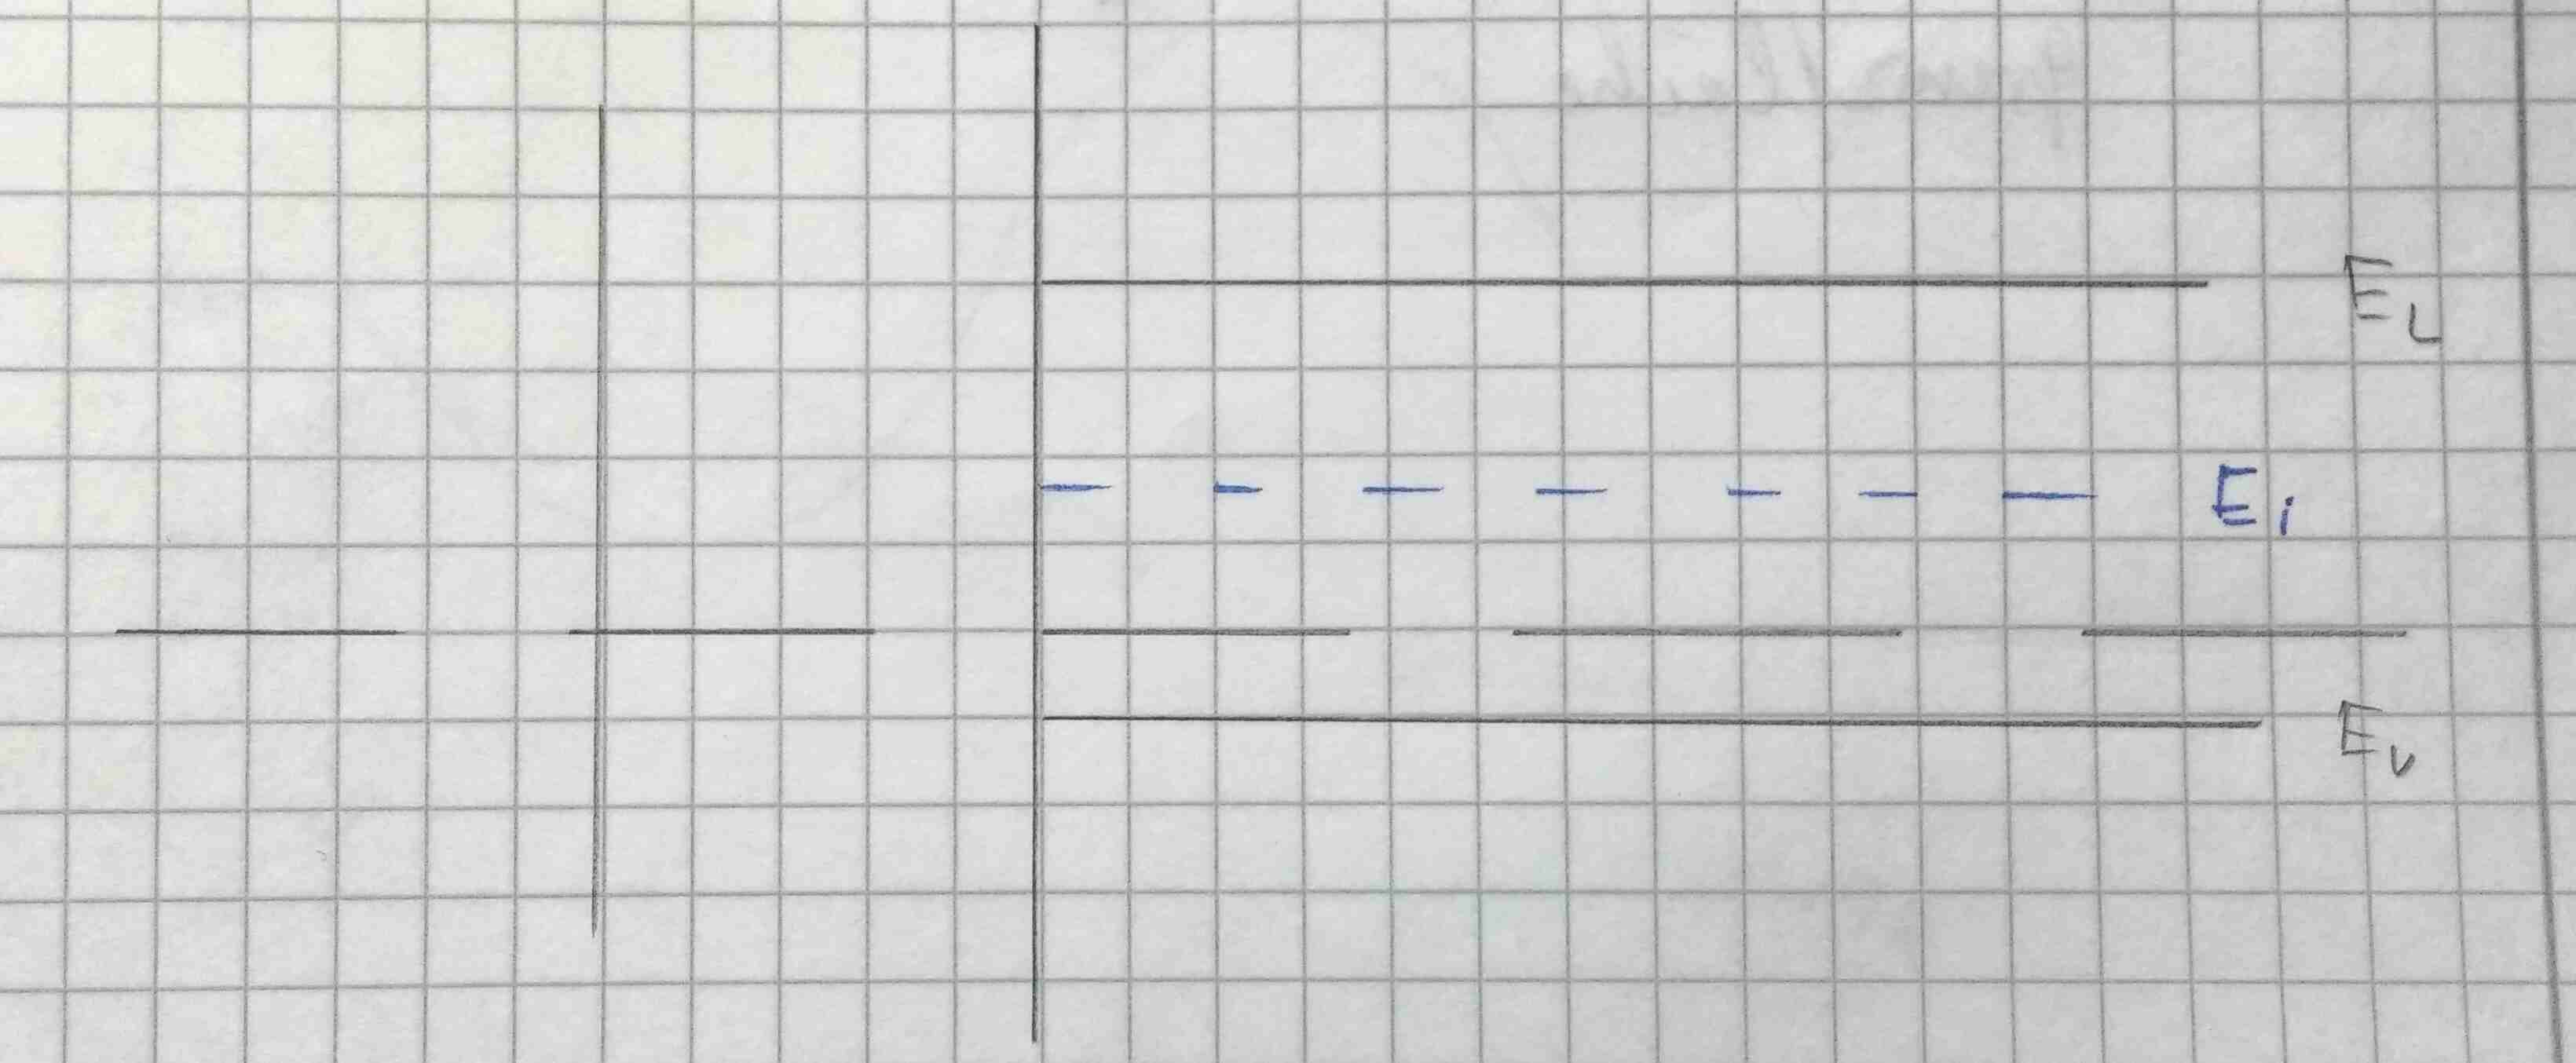
\includegraphics[scale=0.1]{A2_1.jpg}
\end{figure}


\subsection*{c)}

Hier müssen wir einfach in eine Formel einsetzen:

\begin{align*}
N_c &= 2 \cdot \left( \frac{2 \pi \cdot m^* \cdot kT}{h^2} \right)^\frac{3}{2} = 2 \cdot \left( \frac{2 \pi \cdot 0,89 \cdot 9,1 \cdot 10^{-31} \cdot 1,38 \cdot 10^{-23} \cdot 300}{\left( 6,62 \cdot 10^{-34} \right)^2} \right)^\frac{3}{2} = \unit[2,43 \cdot 10^{25}]{m^{-3}}
\end{align*}


\subsection*{d)}

Zunächst ein Bild zu besseren Vorstellung:

\begin{figure}[h]
	\centering
	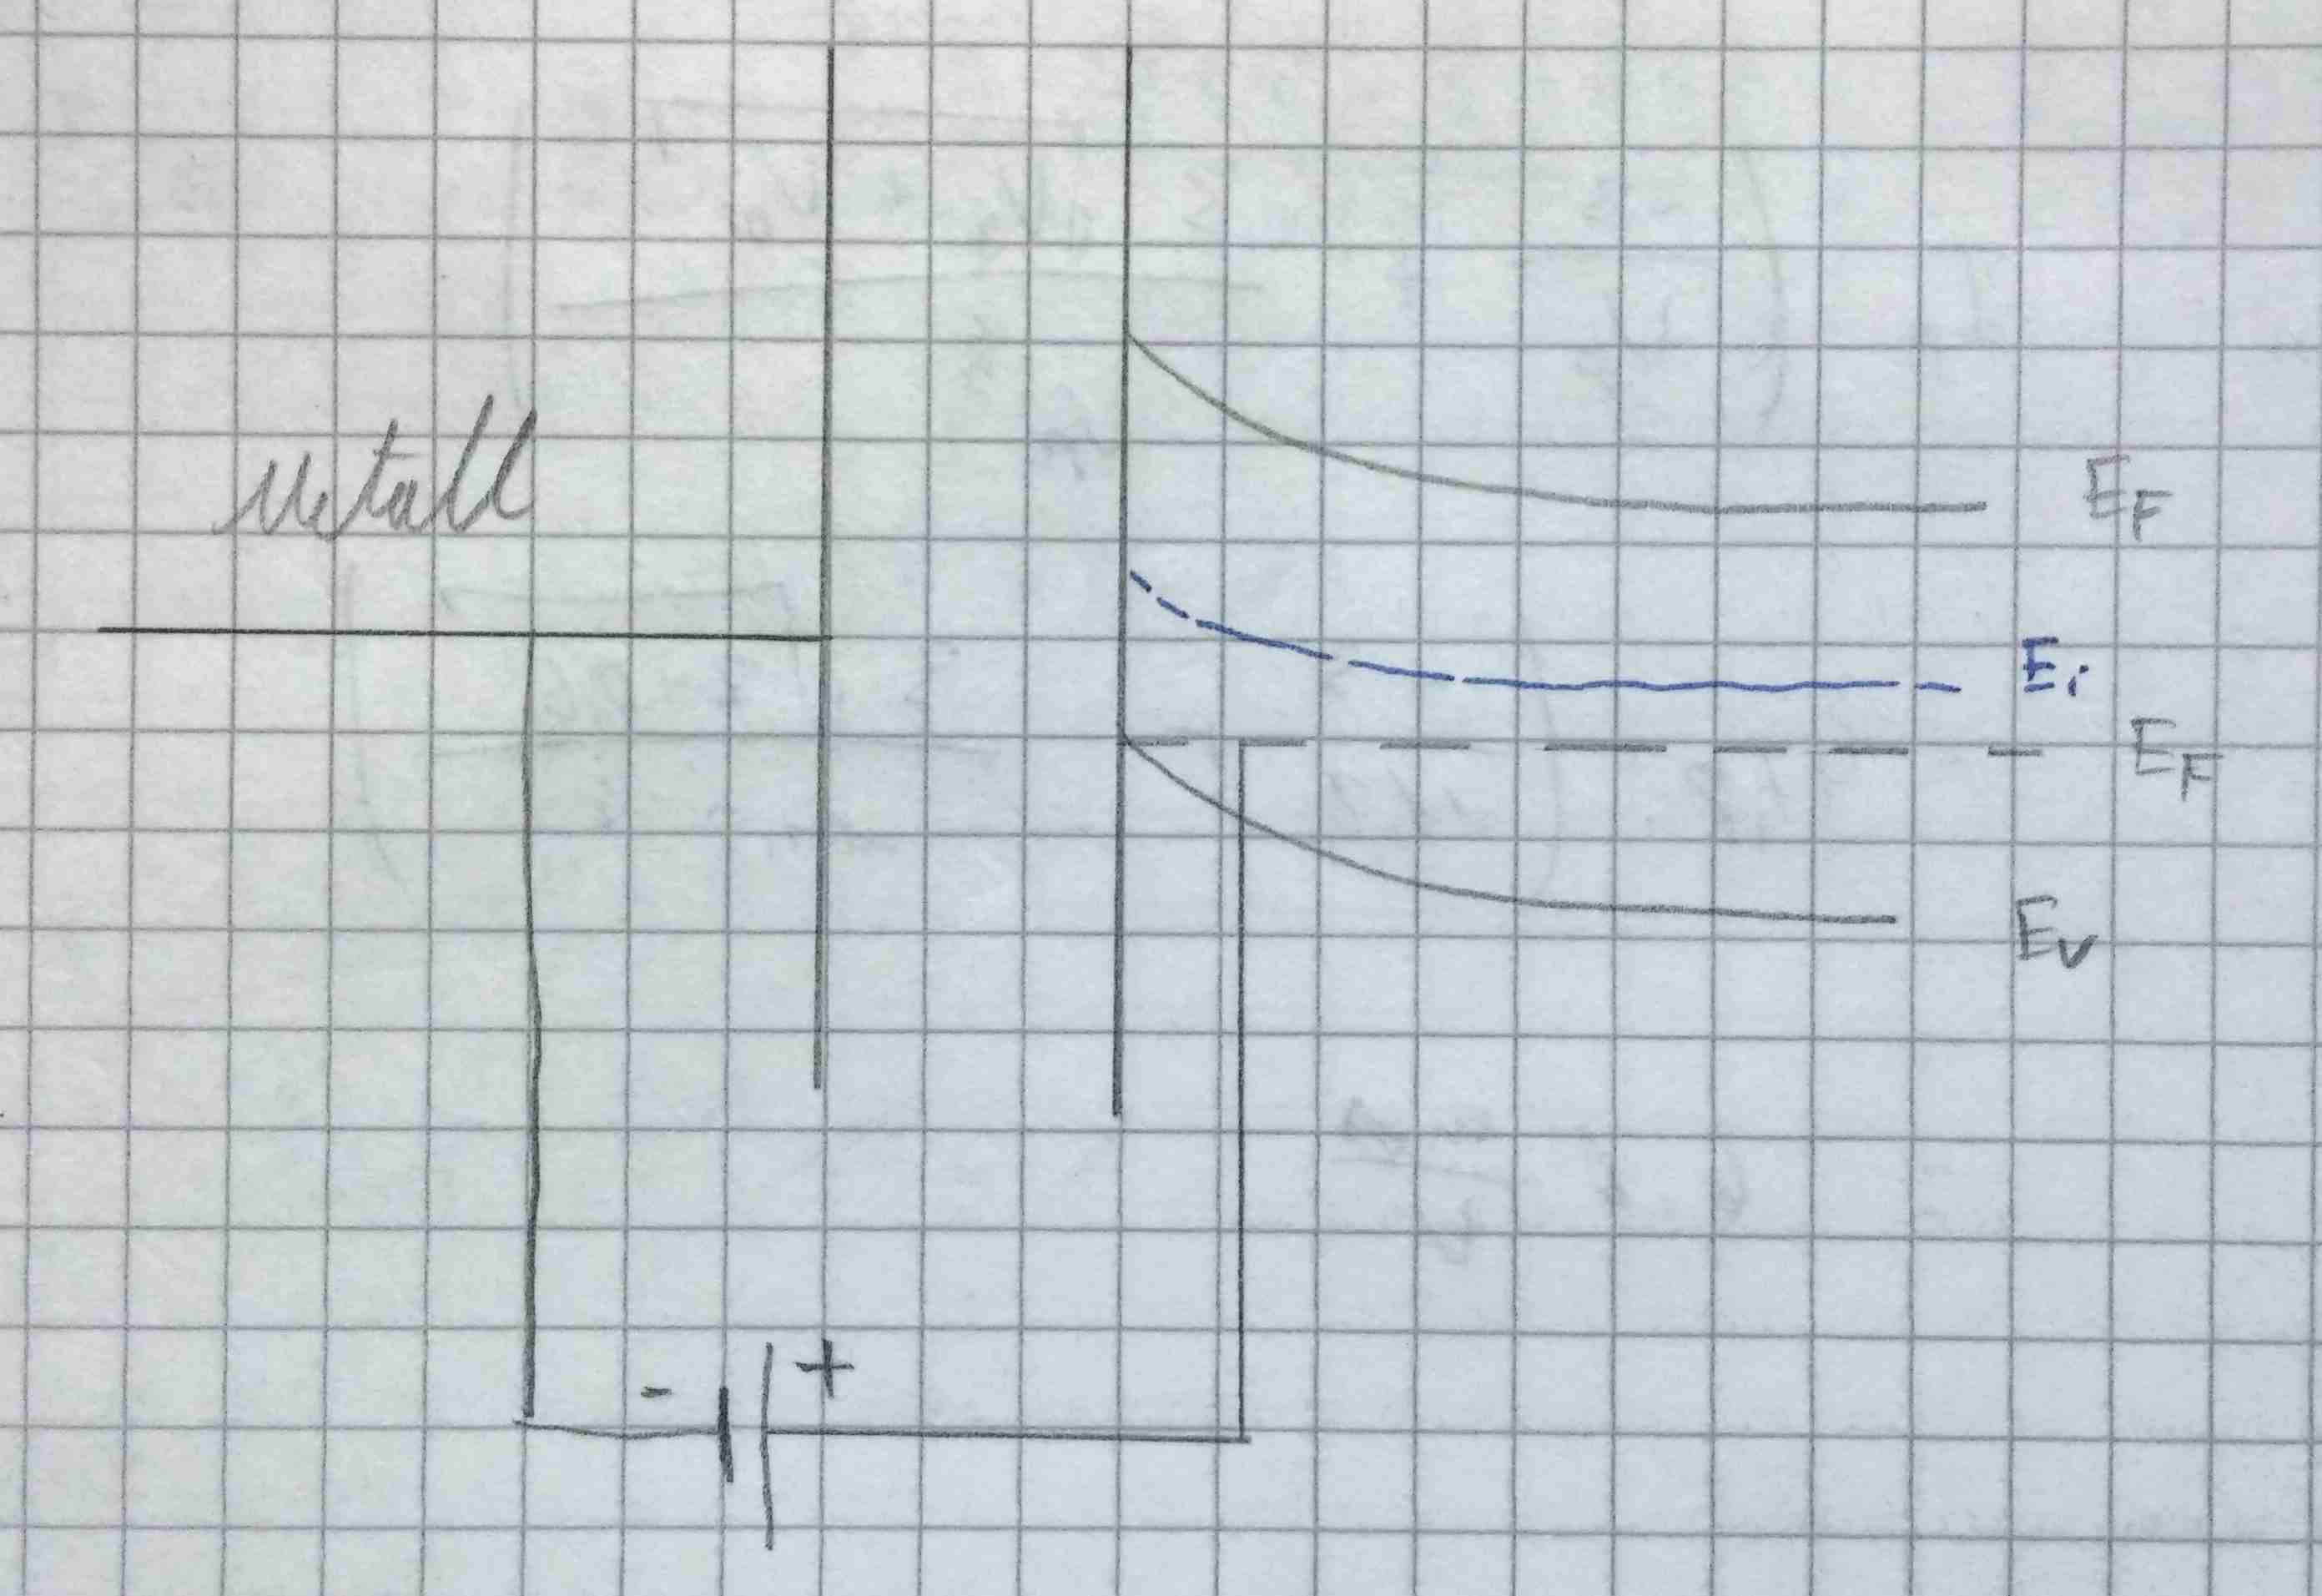
\includegraphics[scale=0.1]{A2_2.jpg}
\end{figure}


Nun setzen wir ein:

\begin{align*}
n &= N_c \cdot e^{- \frac{E_c - E_F}{kT}} = 2,43 \cdot 10^{25} \cdot e^{- \frac{123}{k \cdot 300}} = \unit[2,14 \cdot 10^{23}]{m^{-3}}
\end{align*}


\subsection*{e)}

In der Übung konnte die Lösung zu diesem Teil leider nicht sinnvoll geklärt werden.


\section{Aufgabe 3}

Diese Aufgabe ist im Skript gelöst. Zu finden ist die Lösung im Kapitel 2.5 Heterostrukturen und Schottky-Kontakt. Das ist Seite 157 in dem Sktipt auf meiner Website.


\section{Aufgabe 4}


Die Dicke der Schicht können wir so berechnen:

\begin{align*}
w &= \sqrt{\frac{2 \cdot \epsilon_r \cdot \epsilon_0 \cdot \left( V_{bi} + V_R \right)}{e \cdot N_d}} \qquad \text{Dabei ist  $V_R$ die Gatespannung mit - am Gate}
\intertext{Die Kapazität können wir so bestimmen:}
C &= \frac{\epsilon_0 \cdot \epsilon_r \cdot A}{d} = \frac{\epsilon_0 \cdot \epsilon_r \cdot A}{w} \\
\Rightarrow C' &= \frac{C}{A} = \frac{\epsilon_0 \epsilon_r}{w} = \sqrt{\frac{e \cdot N_d \cdot \epsilon_0 \epsilon_r}{\left( V_{bi} + V_R \right)^2}}
\intertext{Zudem gilt:}
\frac{1}{C'^2} \sim V_{bi} + V_R
\end{align*}

Damit können wir jetzt eine Tabelle mit den Werte aufstellen:

\hfill \\

\begin{center}
	\begin{tabular}{c|c|c|c}
		$n/cm^{-3}$ & $w/ nm$ & $V_R$ & $C'/ mF/m^2$ \\ 
		\hline  
	$10^{16}$	& 290 & 0 & 0,39 \\ 
	$10^{16}$	& 890 & 5 & 0,13 \\ 
	$10^{16}$	& $1,2 \cdot 10^{-3}$ & 10 & $93 \cdot 10^{-3}$ \\ 
	$10^{18}$	& 29 & 0 & 3,9 \\ 
	$10^{18}$	& 89 & 5 & 1,3 \\ 
	$10^{18}$	& $0,12 \cdot 10^{-3}$ & 10 & $928 \cdot 10^{-3}$ \\ 	
	\end{tabular} 
\end{center}

\newpage

Als Graphik sieht das dann so aus:

\begin{figure}[h]
	\centering
	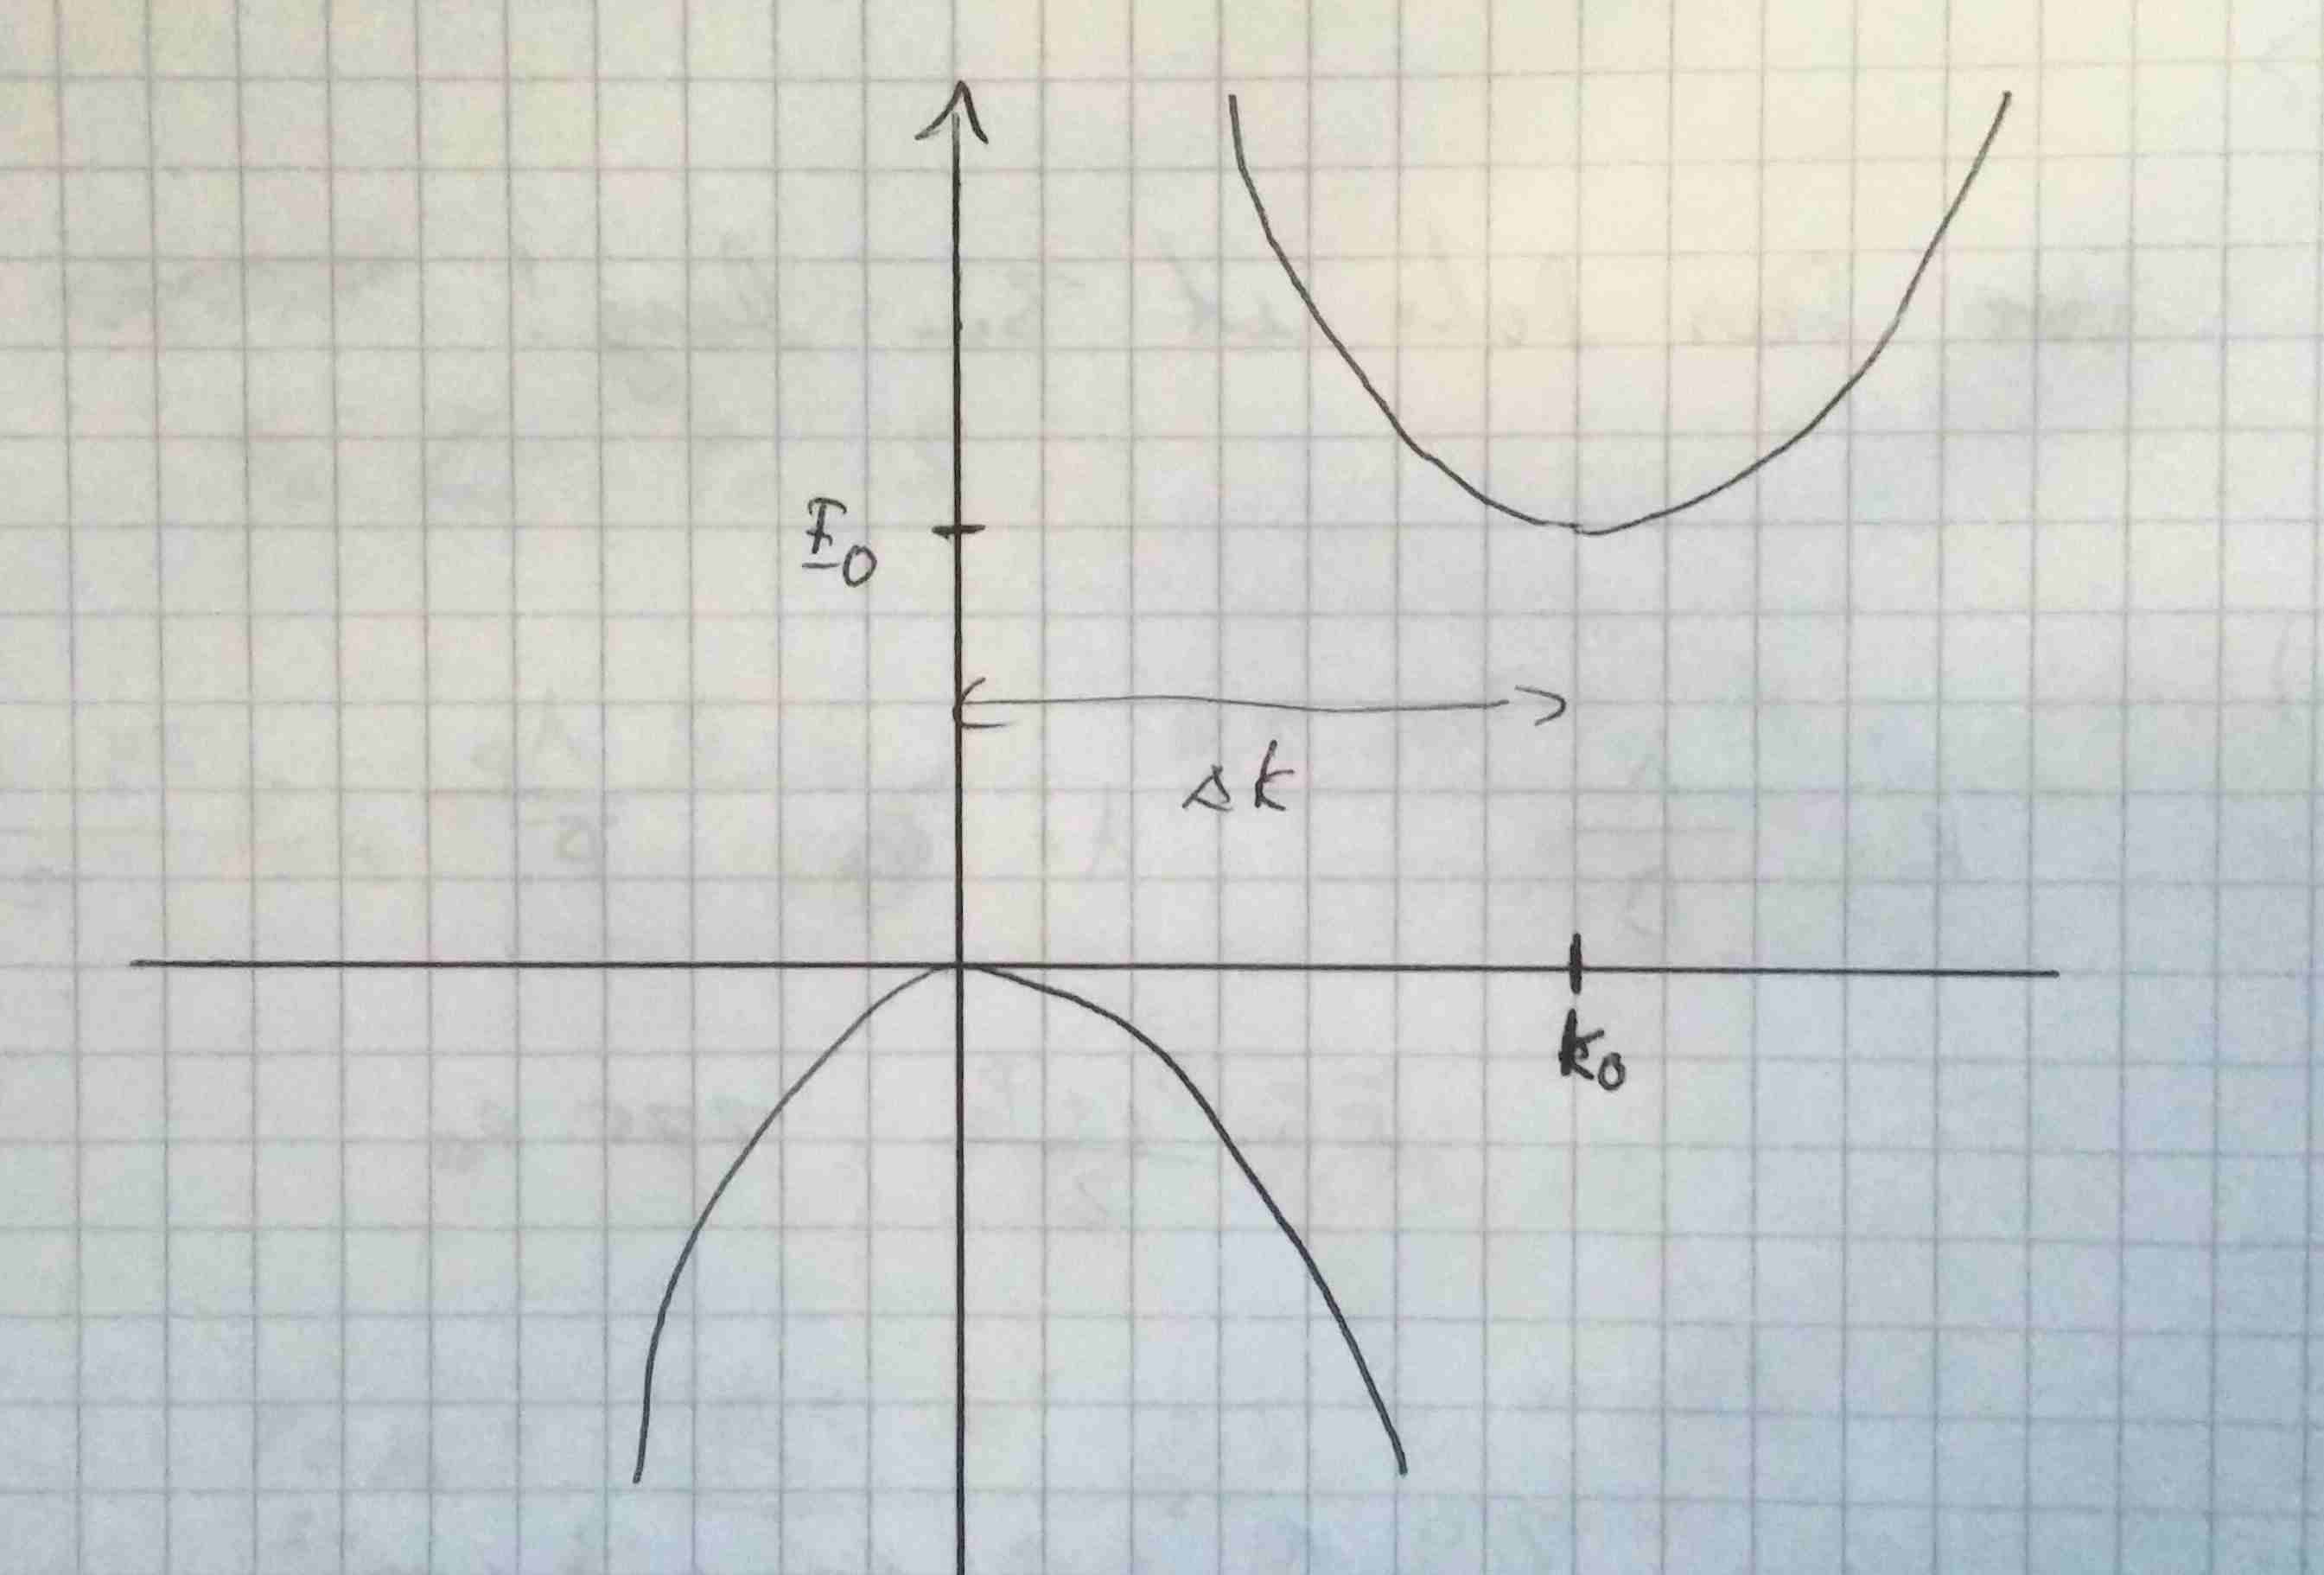
\includegraphics[scale=0.15]{A4_1.jpg}
\end{figure}









 



\end{document}